\chapter{Cardea}\label{sec-cardea}

\section{System Design}
Recalling related works in Chapter 2, what motivates the design of Cardea are the follow:

\begin{itemize}
\item People's privacy concerns are dependent on context. Although in certain circumstances locations are strong hints of possible privacy intrusion, generally what individuals are doing and with whom are more essential and crucial factors that directly relate to privacy.
\item People's privacy preferences vary from each other, thus they should be able to express their personal privacy preferences.
\item People's privacy preferences may change from time to time, therefore they need a way to change such preferences easily.
\end{itemize}

To achieve these objectives, we propose following solution:
\begin{itemize}
\item explain what composes context in Cardea
\item registration of privacy preferences
\item hand gesture for flexibility
\end{itemize}

\begin{table}[tb]
\centering
\caption{Scene categories.}
\label{tbl-scenecate}
\begin{tabular}{ll}
\toprule
Scene category & Scenes                                                  \\ \midrule
Eating         & banquet hall, beer garden, bistro, cafeteria,       \\
               & coffee shop, diner restaurant, food court, sushi bar  \\ \midrule
Entertainment  & ballroom, bar, discotheque, pub                         \\ \midrule
Shopping       & bazzar, clothing store, department store,             \\
               & flea market, florist shop, general store,            \\
               & gift shop, jewelry shop, market, shoe shop,              \\
               & shopping mall, supermarket                           \\ \midrule
Working        & classroom, conference, cubicle, lecture room,           \\
               & library, office, reading room                        \\ \midrule
Public places  & crosswalk, downtown, field road, forest, freeway       \\
               & park, picnic area, street                            \\ \midrule
Transportation & airplane cabin, airport, bus station, bus interior,   \\
               & subway station, train station, railroad track         \\ \midrule
Exhibition     & art gallery, museum                                  \\ \midrule
Religion       & cathedral, chapel, church, mosque, pulpit, temple     \\ \midrule
Illness        & hospital, nursing home                               \\ \midrule
Nudity         & bathroom, beach, coast, lagoon, lavatory,            \\
               & swimming pool, shower, jacuzzi                       \\ \bottomrule
\end{tabular}
\end{table}




\section{Implementation}

\subsection{Scene Classification}

\subsubsection{Data Preparing and Preprocessing}

For scene classification, we use pre-trained model of Places2 dataset provided by~\cite{links:places2mit}. In the time Cardea project was conducted, Places2 dataset provided by the authors contained 401 categories with more than 8 million training images, and the pre-trained model was based on AlexNet structure~\cite{krizhevsky2012imagenet}. By the time this thesis is writing, the dataset is deprecated and the new Places2 dataset contains 365 categories. And the authors provide more pre-trained models based on different network structures~\cite{links:places2pre}.

\begin{figure}[!htbp]
    \centering
    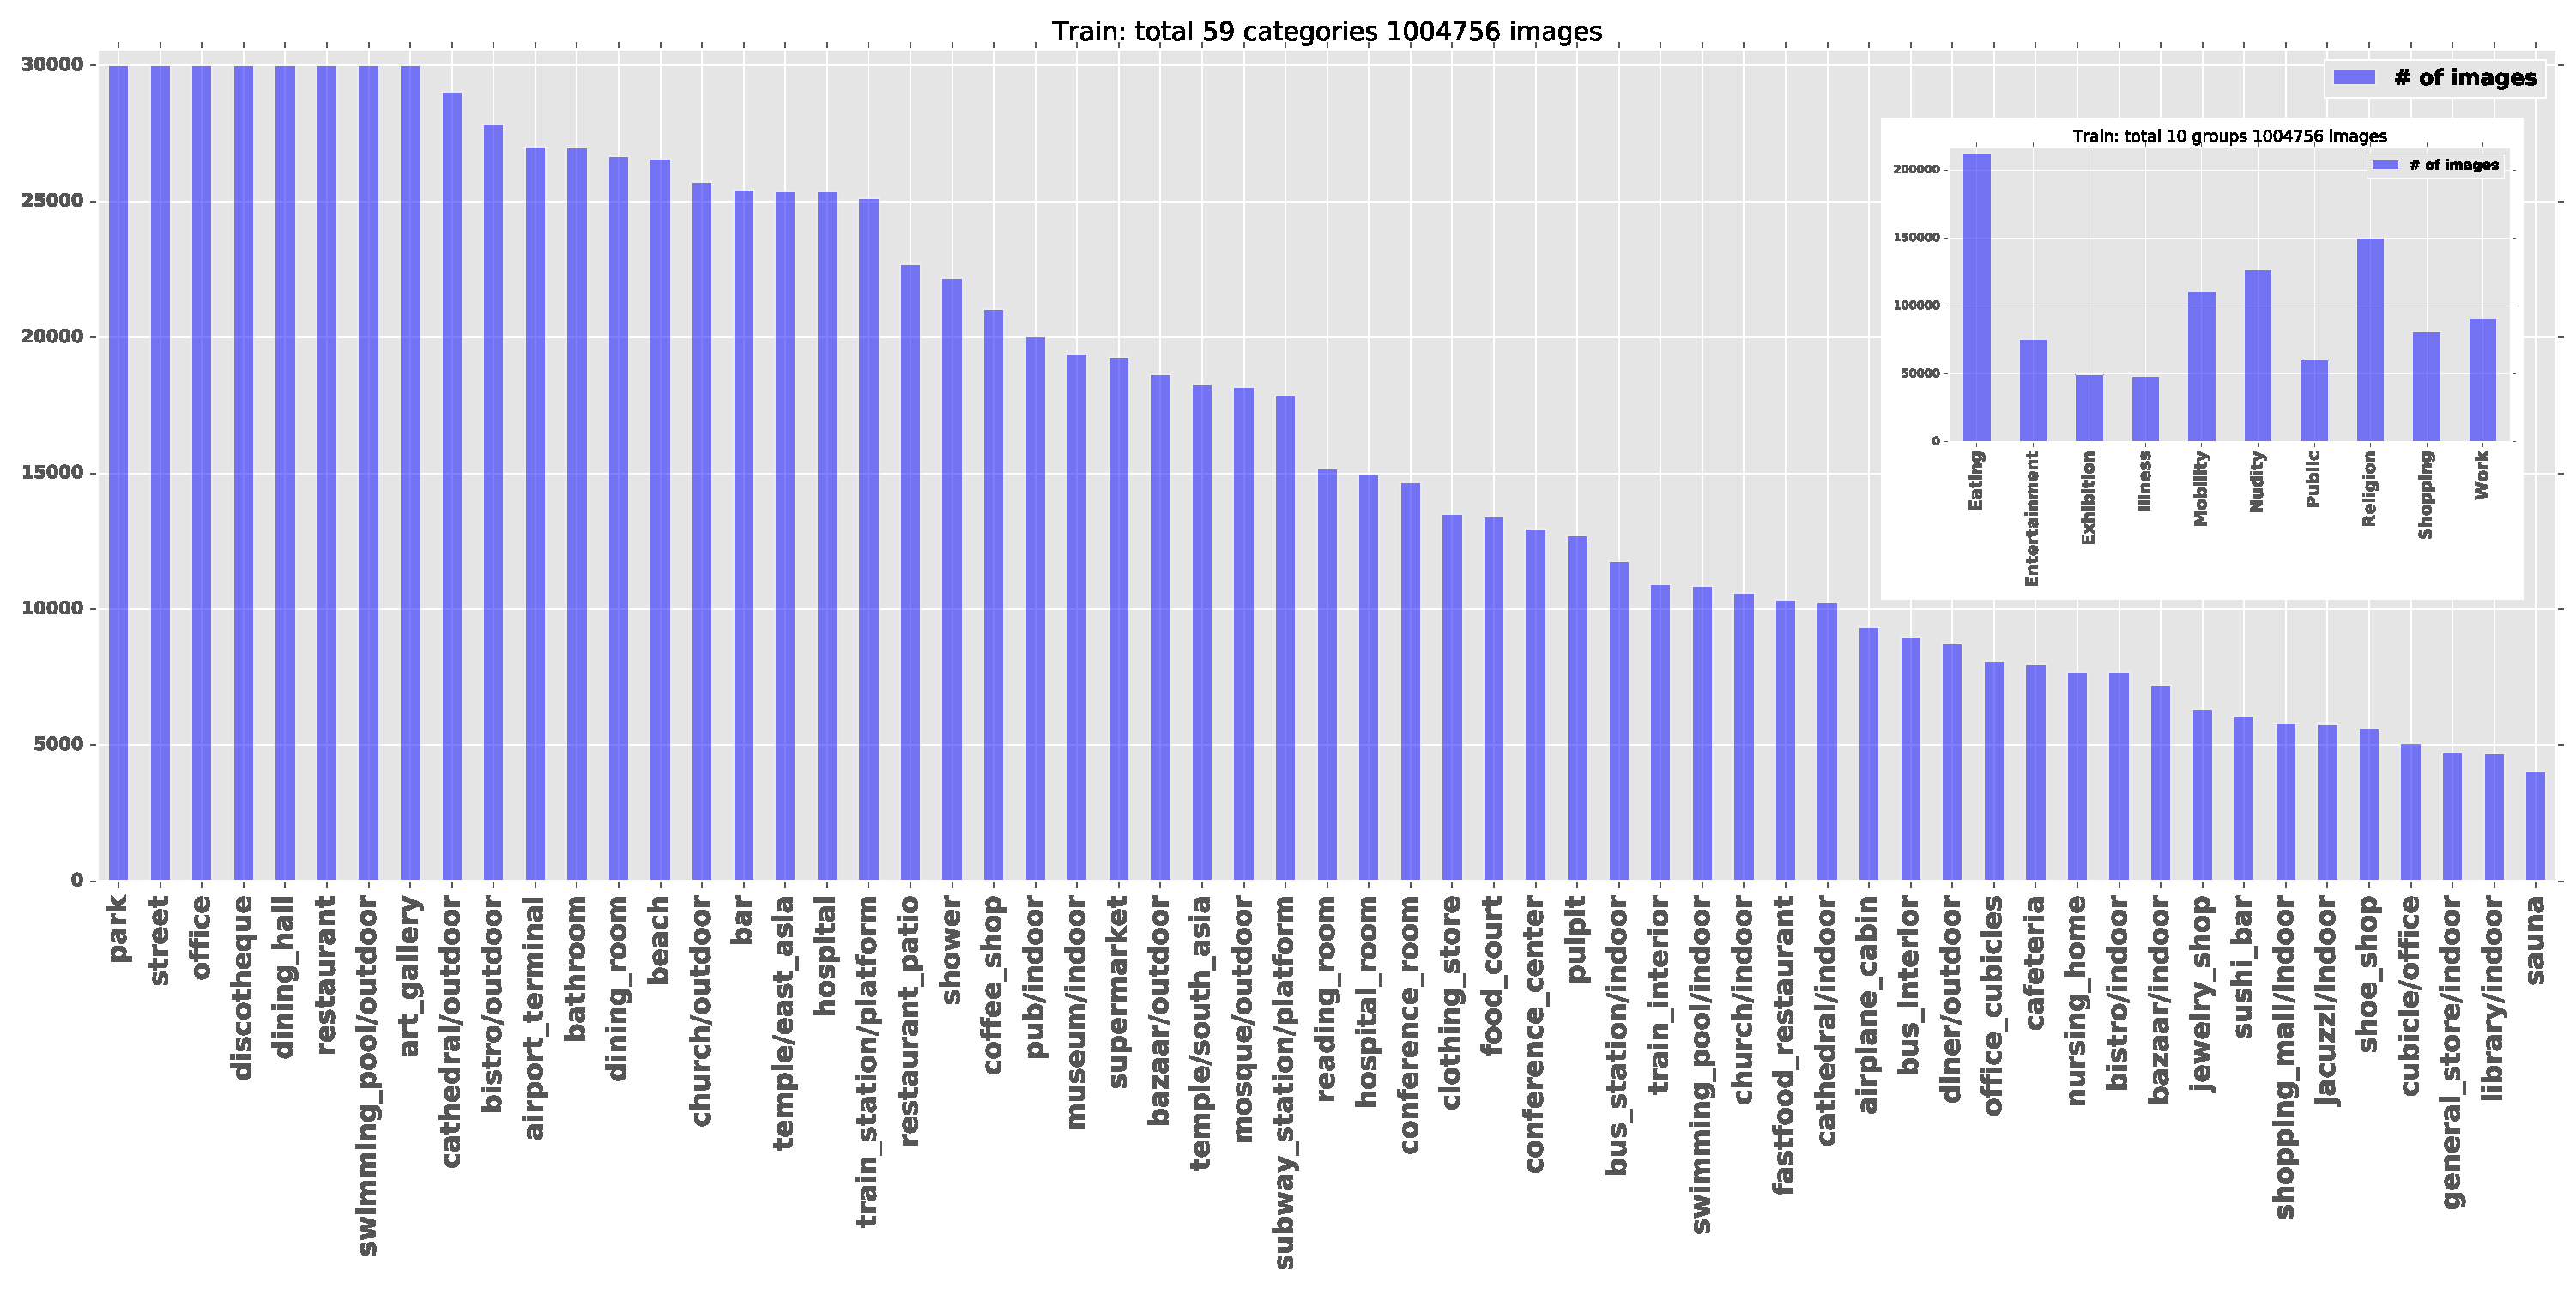
\includegraphics[width=1.0\textwidth]{figure/ch4-numdist.pdf}
    \caption{Number of images for each category and each group (inset).}
    \label{fig:ch4-scenenumdist}
\end{figure}

Note that in the dataset we used, there is a non-uniform distribution of images per category for training, ranging from 4,000 to 30,000, mimicking a more natural frequency of occurrence of the scene. Among the 401 categories, we choose 59 scene categories that are close to daily life and in such scenes people may have privacy concern. In total this subset composed of 1 million training images and 2950 validation images (50 validation images for each category). We also group these 59 scene categories into 10 groups based on contextual similarity, such that people have similar reasons for privacy in scenes that are in the same group (e.g. people don't want to be captured in bathroom and beach is both because of nudity concerns). The distribution of training images among categories and groups is shown in Fig~\ref{fig:ch4-scenenumdist}.

\subsubsection{Training Procedures}
Our training step is just a standard fine-tuning process, which is extensively used in transfer learning~\cite{sharif2014cnn,yosinski2014transferable}:

\begin{itemize}
\item[\ding{182}] Using pre-trained model as feature extractor, we extract the features at \emph{fc7} layer for images belonging to the 59 picked categories. Other than shuffling the features, we also augment the features such that all categories have same amount of features. Though the natural frequencies of occurrence are obviously different among different scenes, we argue that for the purpose of privacy protection, all the scene categories should be equally important, thus categories imbalance is not what we favored. The augmentation step can be implemented using weighted loss layer, but we take simple way of bootstrapping features for categories with less images. After this step, all features are cached and stored in lmdb format.
\item[\ding{183}] Train a softmax classifier of the 59 categories using the extracted features. We choose to train a classifier for categories and then add up the output probabilities to predict the group, rather than directly train a group classifier, is because category classifier tells more about the image, and our desired property is equal weights among scene categories rather than groups.
\item[\ding{184}] Both feature extraction and classifier training are implemented using Caffe library~\cite{links:caffelib,jia2014caffe}. In this step we merge the feature extraction part of pre-trained model and the softmax classifier into a single model by copying weights. Now Caffe has the option of specifying layers with fixed weights, thus simplifying the fine-tuning and deployment process.
\end{itemize}

Other than improving the validation accuracy from 0.56 to 0.57, shuffling also makes training converges faster. With augmentation to relieve category imbalance issue, the classifier can finally achieve 0.600 validation accuracy on the 59 categories. There is no other benchmarking result specifically on the subset we choose, but recent benchmark gives 53\%-56\% validation accuracy on the new Places2 dataset with 365 categories~\cite{links:places2pre}, suggesting our model is competitive. The higher validation accuracy of our model is due to the smaller scale of classification problem we are dealing with.

\subsubsection{Prediction}

\begin{figure}[!htbp]
    \makebox[\textwidth]{
        \centering
        \raisebox{-0.5\height}{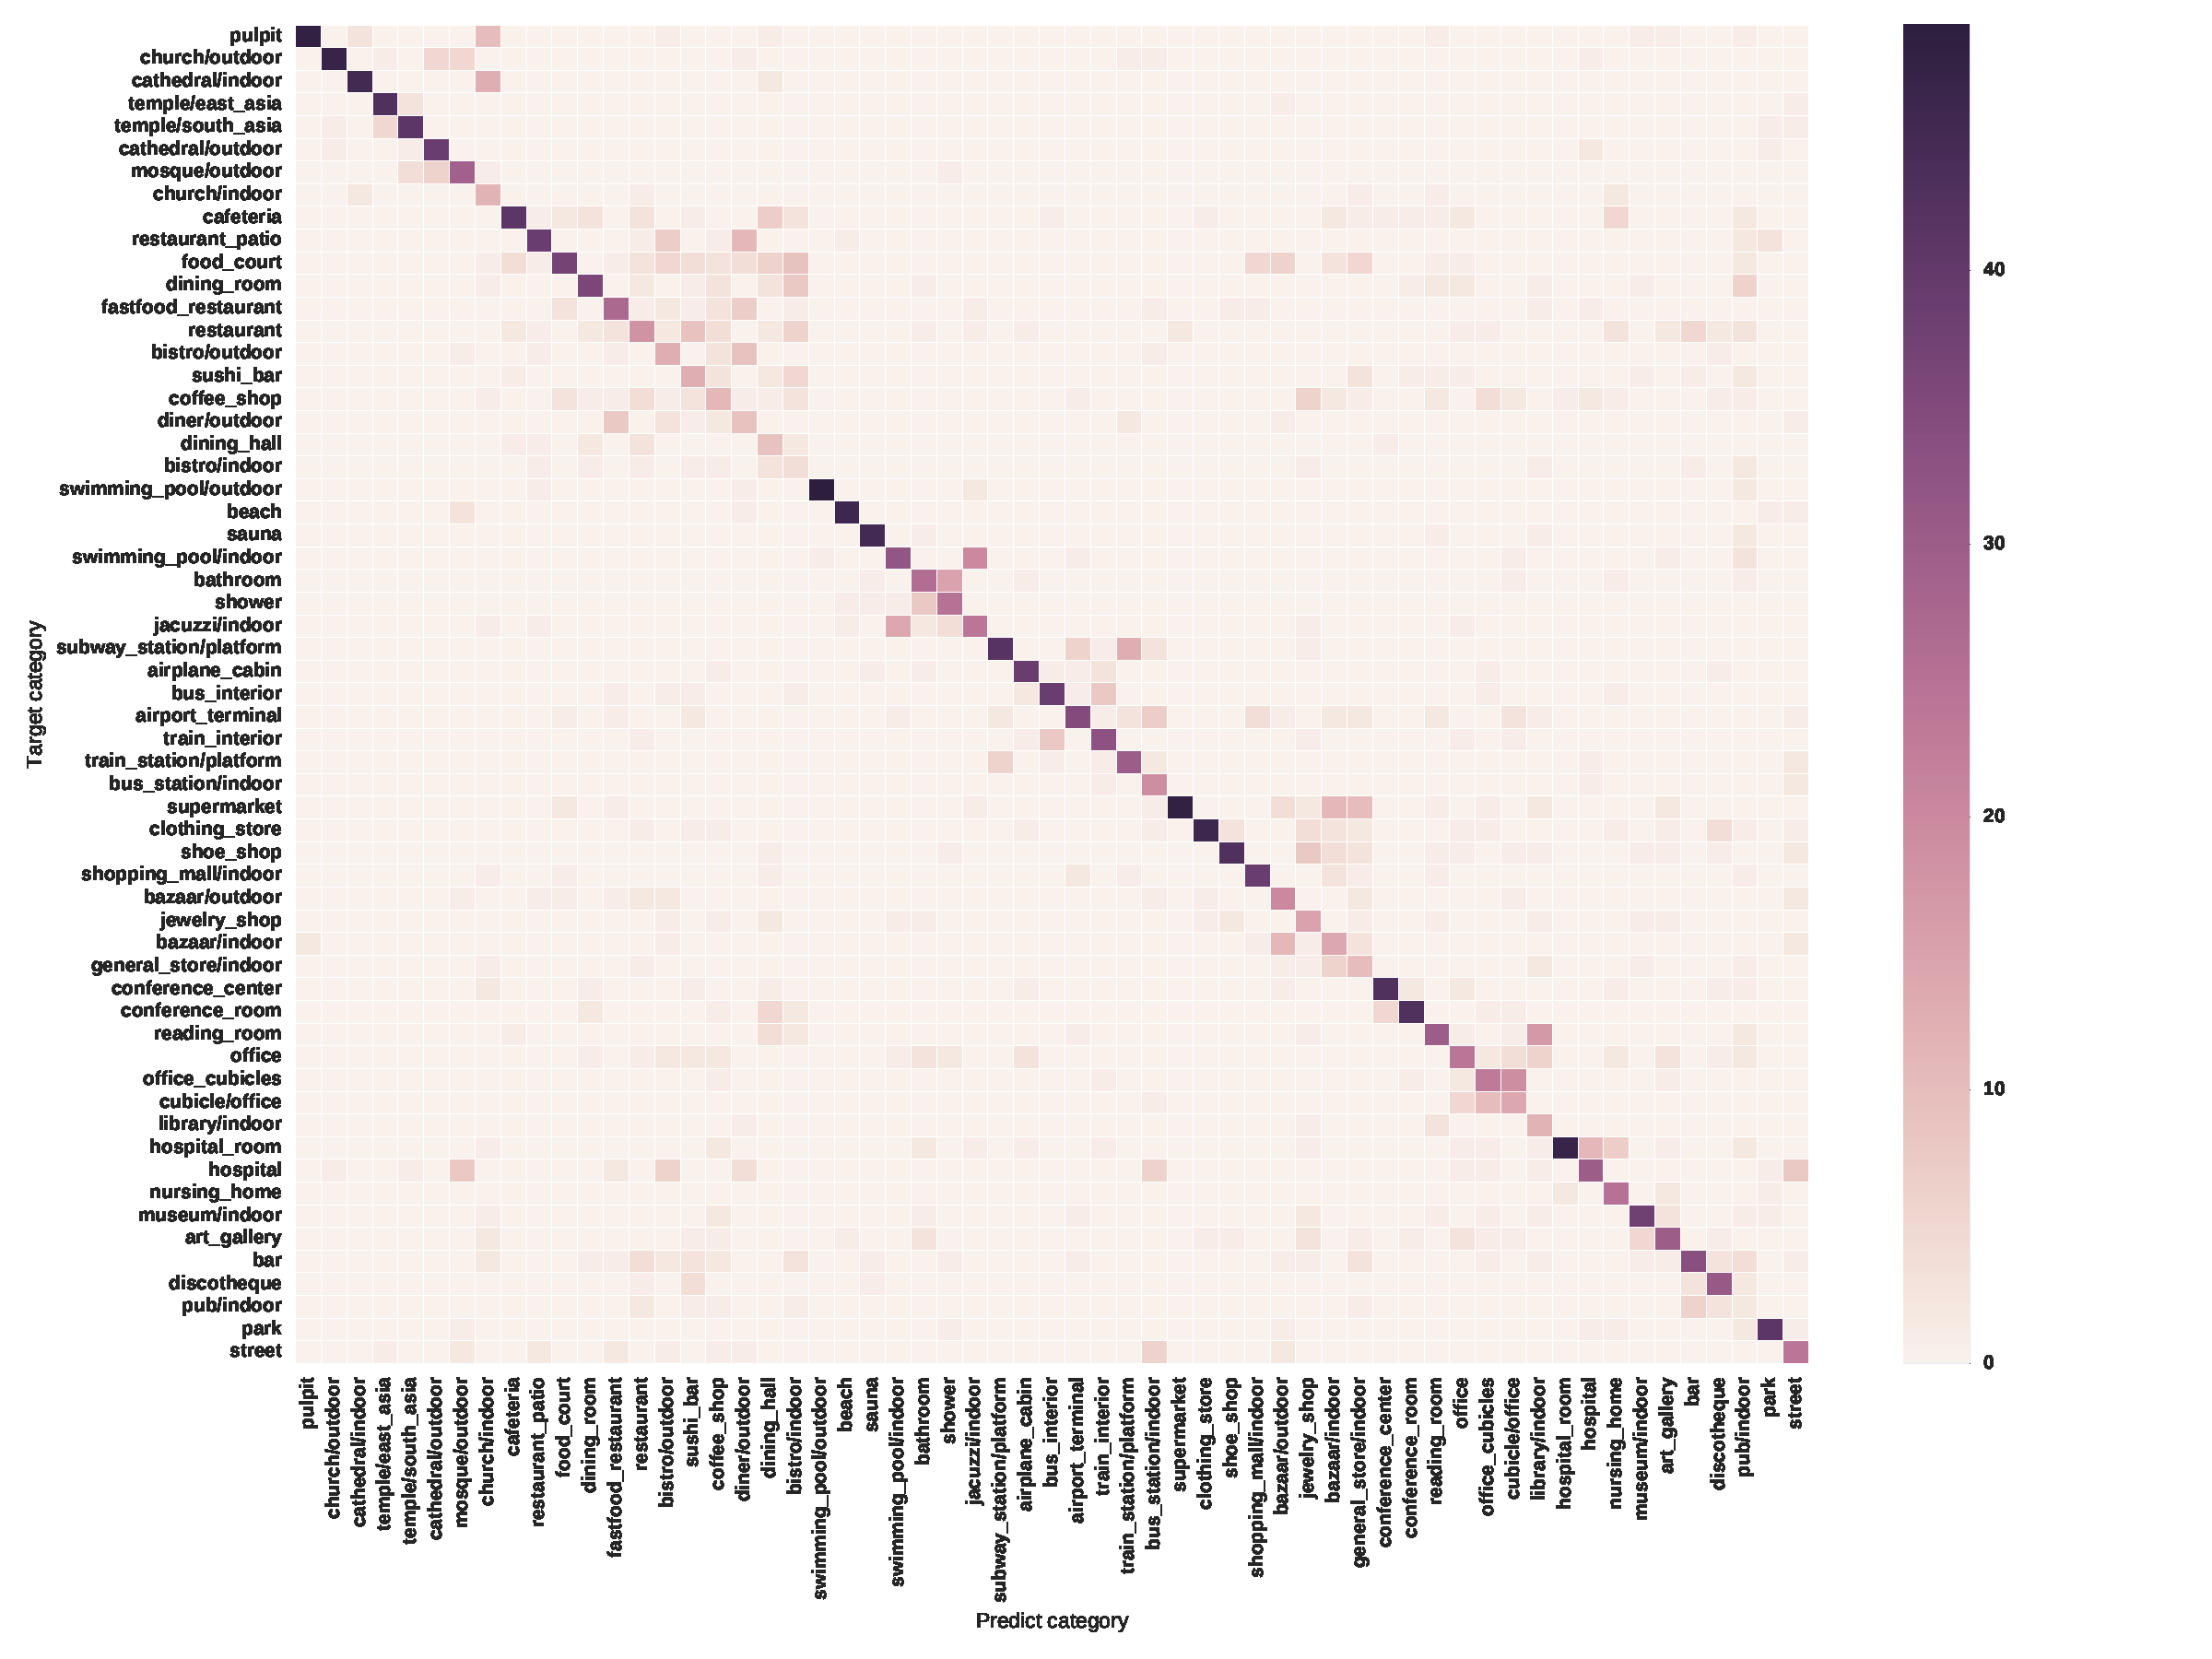
\includegraphics[width=0.7\textwidth]{figure/ch4-scnCateConfu.pdf}}
        \hspace{-1cm}%
        \raisebox{-0.5\height}{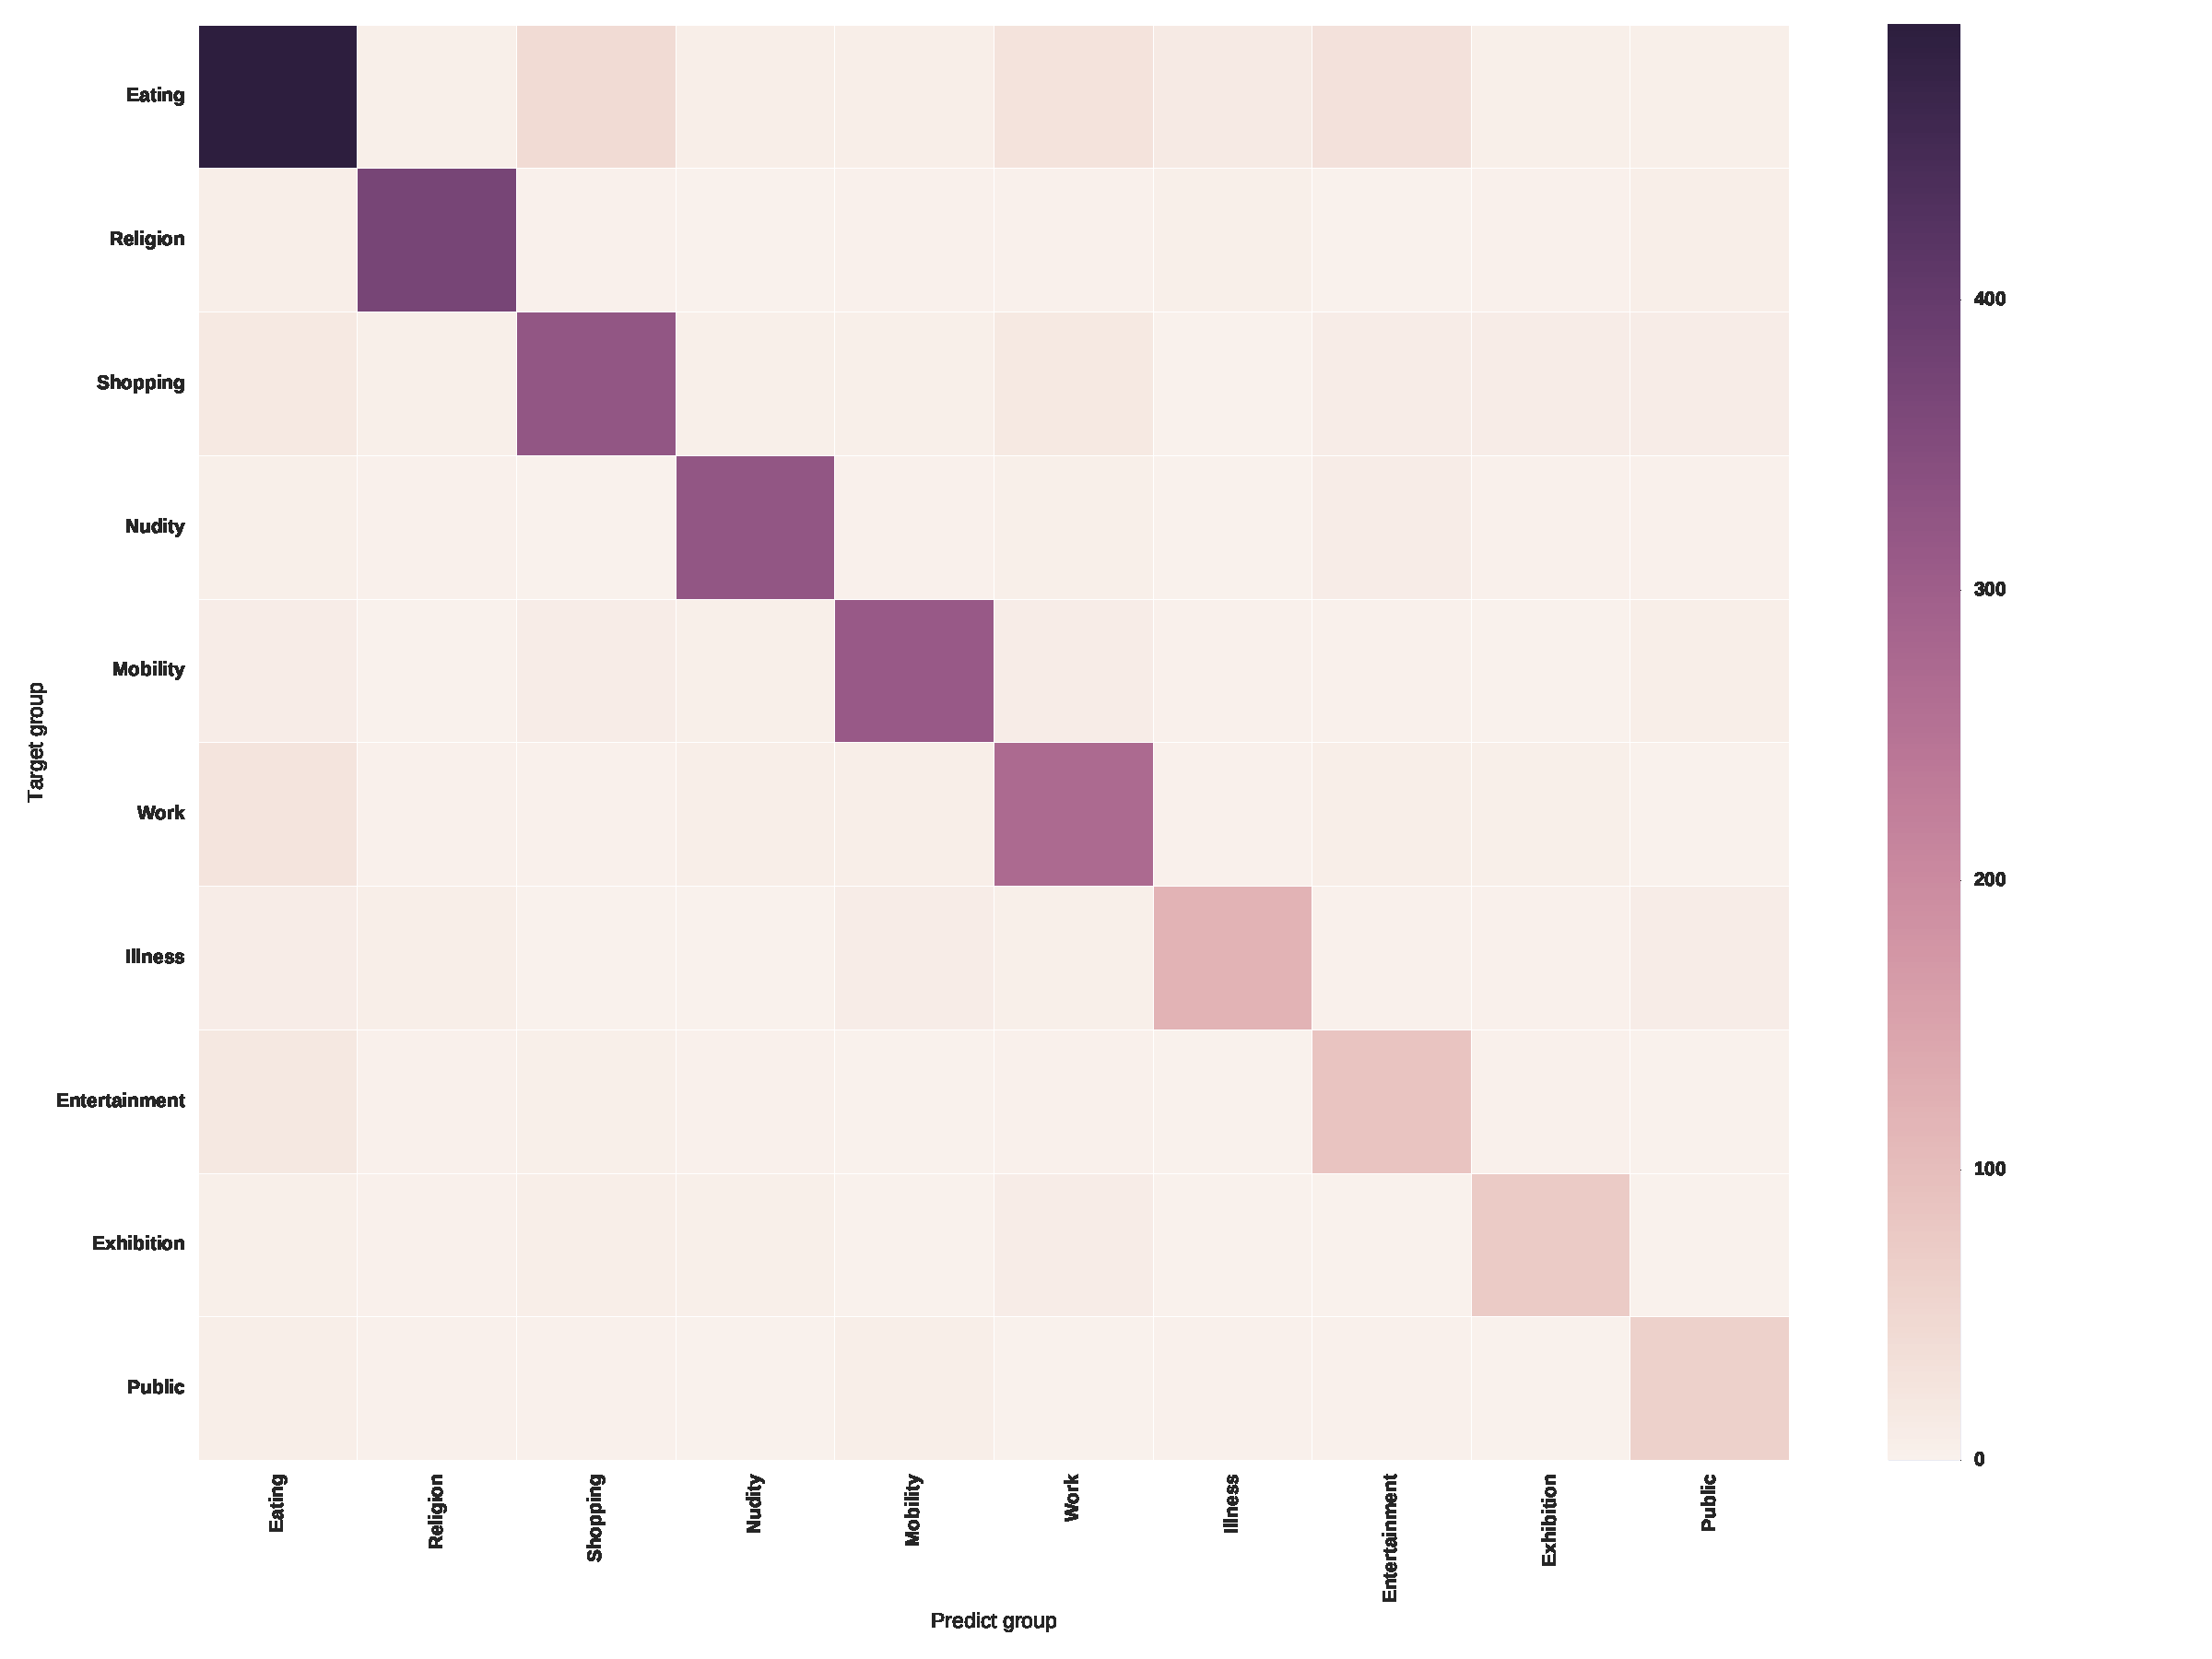
\includegraphics[width=0.6\textwidth]{figure/ch4-scnGrpConfu.pdf}}
    }
    \caption{Confusion matrices for category prediction (left) and group prediction (right).}
    \label{fig:ch4-scnconfumat}
\end{figure}

For prediction, we get probability of a group by summing up the probabilities of all categories belonging to this group, and output the most probable group as prediction of an image. Our model's group prediction accuracy for the validation set is 82.8\%. Fig~\cite{} shows some prediction examples. As seen from the examples, given an image, the predicted category probabilities are usually stratified to few categories within same group, thus group prediction is resilient to perturbation of category prediction. The way we group categories can be seemed as a hard-coded clustering step, which makes prediction more robust to noise. The failure cases are mostly due to natural context ambiguity from a image (e.g. image with object in focus, therefore not enough hints for scene inference). Labeling the 342 non selected categories as extra group will amplify the ambiguity issue, even for images with less ambiguity, doing so will stratify probabilities to the extra group and lead to wrong prediction. In other words, a 59 way classifier leads to higher recall for selected scenes and grouping leads to higher accuracy. This is also reflected in confusion matrices shown in Fig~\ref{fig:ch4-scnconfumat}, category confusion matrix shows some clustering structure which is in accordance with the groups we manually assigned. However, only using top 1 category for prediction sacrifices prediction accuracy, which can be avoided by grouping as shown in group confusion matrix.


\subsection{Face Recognition}
Like scene classification, we select a pre-trained model for face recognition task. More specifically, the pre-trained model will serve as face feature extractor, and we will update the face classifier whenever new users register in Cardea and upload their face features. There are already many deep neural networks deployed in commercial products, like Megvii's Face++~\cite{zhou2013extensive}, Facebook's Deepface~\cite{taigman2014deepface}, Google's Facenet~\cite{schroff2015facenet}, Sensetime's Deepid~\cite{sun2015deepid3}. OpenFace~\cite{amos2016openface} is an open source project that is gaining attentions in recent months, it is based on Torch~\cite{links:torch7}. Because Cardea's other modules are under Caffe framework, we limit our options on open sourced Caffe models. The models in our consideration are VGG face recognition model~\cite{parkhi2015deep} and Lightened CNN face recognition model~\cite{wu2015lightened}.

\begin{figure}[!htbp]
    \makebox[\textwidth]{
        \centering
        \raisebox{-0.5\height}{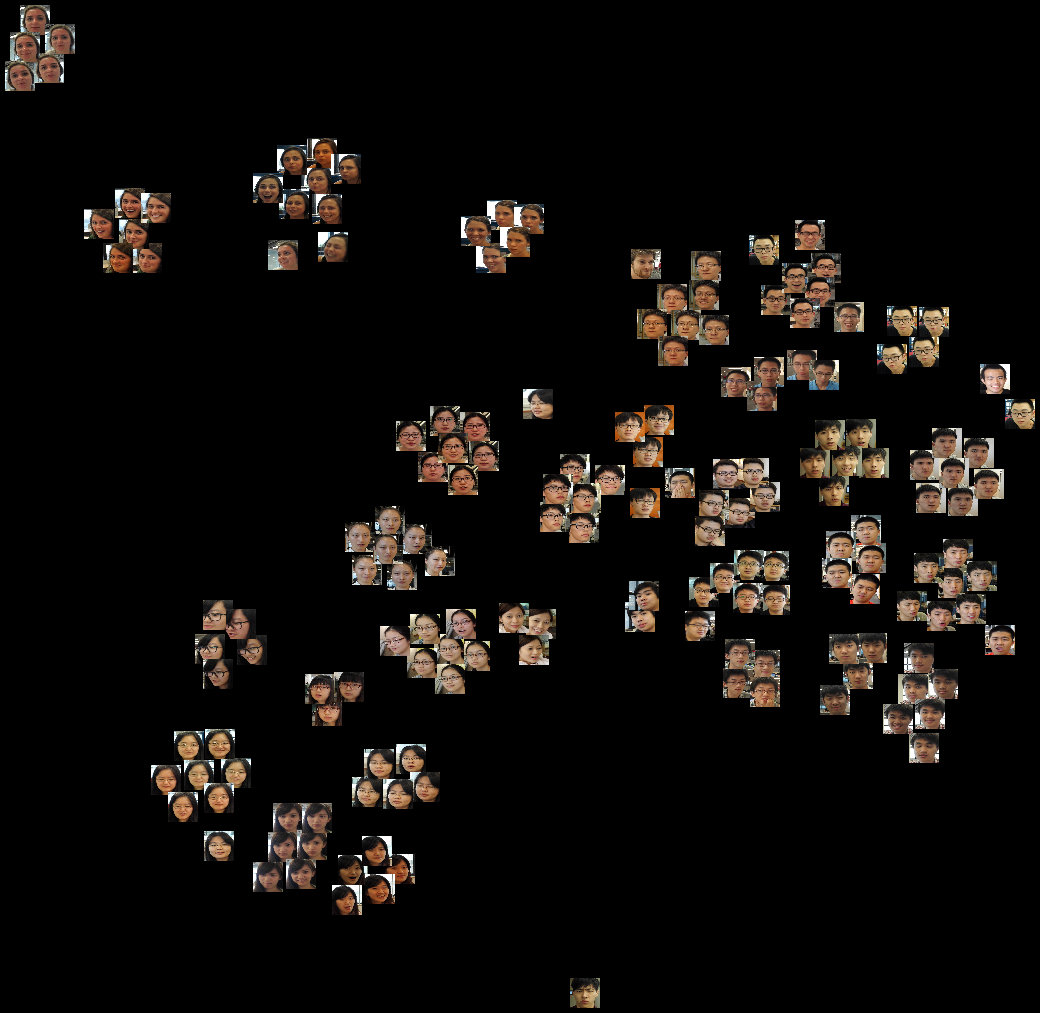
\includegraphics[width=0.6\textwidth]{figure/ch4-tsnevggfc8.png}}
        \raisebox{-0.5\height}{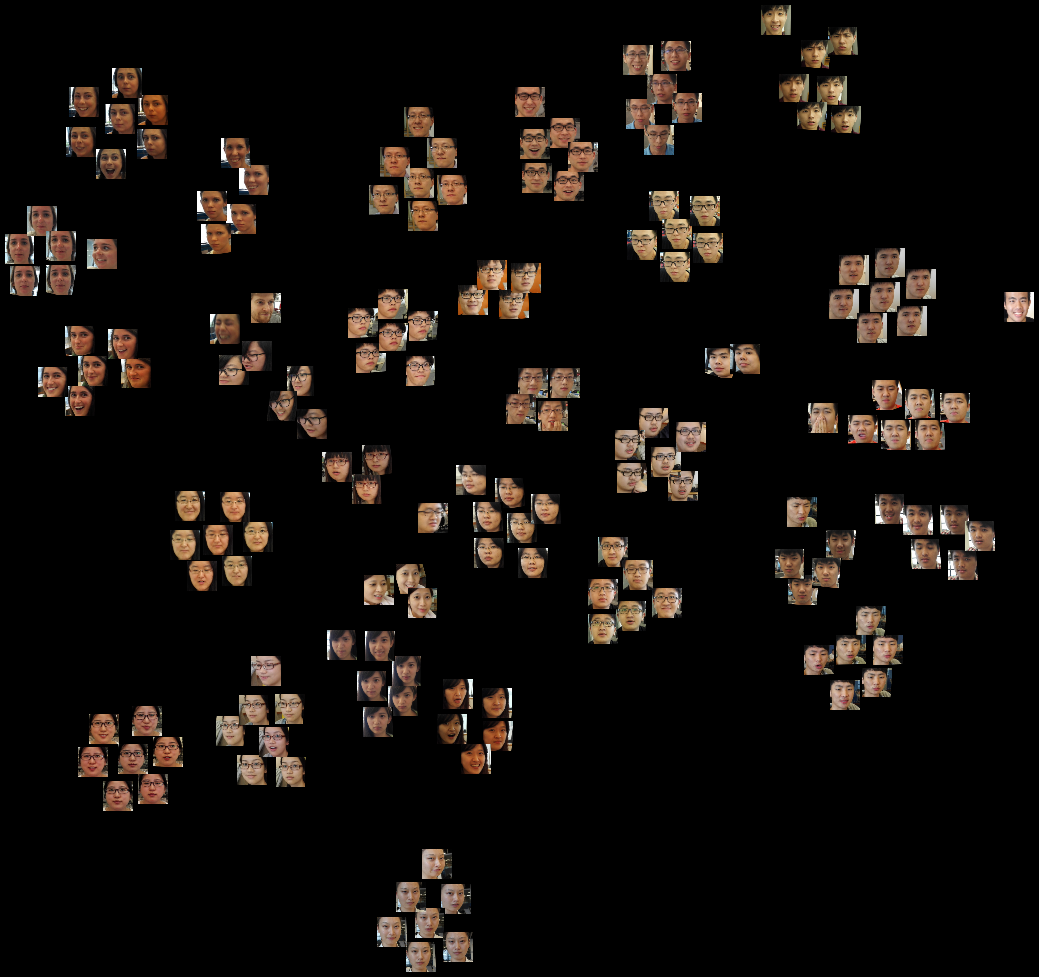
\includegraphics[width=0.62\textwidth]{figure/ch4-tsnemfmeltwise_fc1.png}}
    }
    \caption{t-SNE visualization of VGG \emph{fc8} layer features and Lightened CNN \emph{fc1} layer features.}
    \label{fig:ch4-tsnevggvsmfm}
\end{figure}

To compare performance of features extracted from the two models, we run t-SNE visualization~\cite{maaten2008visualizing} on the features of a small dataset we previously collected for emotion sensing. Fig~\ref{fig:ch4-tsnevggvsmfm} shows the t-SNE visualization result. It seems VGG feature and Lightened CNN feature have similar performance, at least on this small dataset. Though it is found that comparing to Lightened CNN model, VGG model is more robust to variations and its features show better transferability~\cite{ghazi2016comprehensive}, the model size is more than 500MB, 10 times bigger than Lightened CNN model. And the released VGG model has a feature dimension of 4096, while Lightened CNN model has a feature dimension of 256. Our experiment on different Android smartphones shows it takes 10 times longer to extract VGG features. Table~\ref{tbl-forwardingtime} shows the forwarding time we tested on different smartphones. It can be seen VGG model consumes much more memory that it can only run on phones with memory larger than 3GB. Due to above concerns, we use Lightened CNN model in our implementation.

\begin{table}[tb]
\centering
\caption{Time of single facial feature extraction and batch facial feature extraction (10 faces).}
\label{tbl-forwardingtime}
\begin{tabular}{lrrr}
\toprule
 & Xiaomi Mi 3W & Galaxy Note 4 & Xiaomi Mi 5\\
 & {\small Snapdragon 800} & {\small Snapdragon 805} & {\small Snapdragon 820}\\
 & {\small 2GB RAM} & {\small 3GB RAM} & {\small 4GB RAM}\\
 \midrule
1 VGG CNN & N/A & N/A & $\sim 2780$ ms \\
10 VGG CNN & N/A & N/A & $\sim 26740$ ms \\
1 Lightened CNN & $\sim 508$ ms & $\sim 330$ ms & $\sim 303$ ms \\
10 Lightened CNN & $\sim 6602$ ms & $\sim 3971$ ms & $\sim 2031$ ms \\
 \bottomrule

\end{tabular}
\end{table}


\subsubsection{Detection and Alignment}
Lightened CNN model takes aligned face as input, requiring that the distance between midpoint of eyes and midpoint of mouth is 48, and $y$ value of midpoint of eyes is 40, as shown in Fig~\ref{}. We use OpenCV's haar cascade~\cite{links:opencv,viola2001rapid} frontal face detector. The limitation it brings to Cardea is only frontal faces will be detected and recognized. We set \emph{minNeighbors} (the parameter specifying how many neighbors each candidate rectangle should have to retain it) to be 3 to ensure a relative high recall for face detection. To remove false positive, we further apply skin color filter (range $[0, 48, 60] - [30, 255, 255]$ in HSV color space) on retained rectangles. Following that, we use Dlib library's HOG~\cite{links:dlib,dalal2005histograms} based face detector as a second stage filter. Note that Dlib's face detector has higher accuracy comparing to OpenCV's face detector, but is much slower if applied directly on a high resolution image, therefore it is used as a filter on small rectangular areas. Dlib's facial landmarks detector~\cite{links:dlibfacepose} is also used in later face alignment stage, it can detect 68 facial landmarks~\cite{links:dlibfacelandmarkspos, links:dlibfacelandmarkscoords}. With the detected landmarks and required alignment condition about inputs to the CNN model, we can calculate the homography matrix that is finally used to align faces. The steps for detection and alignment is shown in Fig~\ref{}, and we implemented it as a JNI library for Android platform~\cite{links:facealignjni}.

{\bfseries add figure for detection and alignment steps}

\subsubsection{Face Matching}


\subsection{Gesture Recognition}


\subsection{Deployment on Android}

forwarding time

\subsection{System Integration}

data flow

screen shots

decision tree



\subsection{Overview}
technical focus , final object is to prove feasibility of proposed solution, shed lights on future explorations

\section{Evaluation}


\newpage
